\documentclass[journal,10pt,twocolumn]{article}
\usepackage{graphicx, float}
\usepackage[margin=0.5in]{geometry}
\usepackage{amsmath, bm}
\usepackage{array}
\usepackage{booktabs}
\usepackage[utf8]{inputenc}
\usepackage{amsfonts}
\usepackage{amssymb}
\usepackage{graphicx}
\usepackage{multicol}
\usepackage{tabularx}
\usepackage{hyperref}
\DeclareUnicodeCharacter{2212}{-}
\providecommand{\norm}[1]{\left\lVert#1\right\rVert}
\providecommand{\sbrak}[1]{\ensuremath{{}\left[#1\right]}}
\providecommand{\lsbrak}[1]{\ensuremath{{}\left[#1\right.}}
\providecommand{\rsbrak}[1]{\ensuremath{{}\left.#1\right]}}
\providecommand{\brak}[1]{\ensuremath{\left(#1\right)}}
\providecommand{\lbrak}[1]{\ensuremath{\left(#1\right.}}
\providecommand{\rbrak}[1]{\ensuremath{\left.#1\right)}}
\providecommand{\cbrak}[1]{\ensuremath{\left\{#1\right\}}}
\providecommand{\lcbrak}[1]{\ensuremath{\left\{#1\right.}}
\providecommand{\rcbrak}[1]{\ensuremath{\left.#1\right\}}}
\newcommand{\myvec}[1]{\ensuremath{\begin{pmatrix}#1\end{pmatrix}}}
\let\vec\mathbf

\title{\textbf{Circle Assignment}}
\author{YOGEESH REDDY \hspace{9cm} FWC22076}
\date{September 2022}

\begin{document}

\maketitle
\paragraph{\textit{Problem Statement} - The centre of  circle inscribed in square formed by the lines \(x^2-8x+12=0\) and \(y^2-14y+45=0\)  is ?}

\section*{\large Solution}

\begin{figure}[H]
\centering
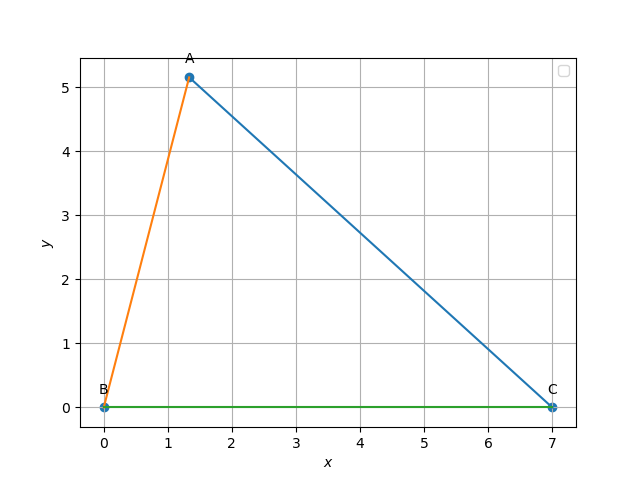
\includegraphics[width=1\columnwidth]{Figure_1.png}

\label{fig:triangle}
\end{figure}
 
The Standard Equations of the Circle are :
    \begin{align}
\vec{x}^{\top}\vec{V_1}\vec{x}+2\vec{u_1}^{\top}\vec{x}+f_1=0
\end{align}  
\begin{align}
\vec{V_1}&=\begin{pmatrix}
	1 & 0\\
	0 & 0\\
	\end{pmatrix} \\
    \vec{u_1}&=\begin{pmatrix}
	-4\\
	0 \\
	\end{pmatrix} \\
	f_1&=12
	\end{align}
	   \begin{align}
\vec{x}^{\top}\vec{V_2}\vec{x}+2\vec{u_2}^{\top}\vec{x}+f_2=0
\end{align}  
	\begin{align}
\vec{V_2}&=\begin{pmatrix}
	0 & 0\\
	0 & 1\\
	\end{pmatrix} \\
    \vec{u_2}&=\begin{pmatrix}
	0\\
	-7 \\
	\end{pmatrix} \\
	f_2&=45
	\end{align}

 
 \vspace{4mm}
The lines in given pairs of straight lines are :

\begin{align}
\vec{m_1}^{\top}\brak{\vec{V_2}\vec{q_1}+\vec{u_2}} = 0
\end{align}
\begin{align}
		e_2^Tx=k_1	
\end{align}
            Yielding,
           \begin{align}
\vec{q_1}=\myvec{2\\7}
\end{align}
            
\begin{align}
\vec{m_1}^{\top}\brak{\vec{V_2}\vec{q_2}+\vec{u_2}} = 0
\end{align}
\begin{align}
		e_2^Tx=k_2	
		\end{align}
		Yielding,
		\begin{align}
\vec{q_2}=\myvec{6\\7}
\end{align}

\begin{align}
\vec{m_2}^{\top}\brak{\vec{V_1}\vec{q_3}+\vec{u_1}} = 0
\end{align}
\begin{align}
		e_2^Tx=k_3
\end{align}
Yielding,
\begin{align}
\vec{q_3}=\myvec{4\\5}
\end{align}
\begin{align}
\vec{m_2}^{\top}\brak{\vec{V_1}\vec{q_4}+\vec{u_1}} = 0
\end{align}
\begin{align}
e_2^Tx=k_4
\end{align}
Yielding,
\begin{align}
\vec{q_4}=\myvec{4\\9}
\end{align}
  The centre of circle is given by:
     \begin{equation}
     \vec{O}=\frac{\vec{q_1}+\vec{q_2}}{2}
          \end{equation}
        
        \begin{equation*}
        \vec{O}=\myvec{4\\7}
\end{equation*}          
    
     
     T
 

\section*{\large Construction}
{
\setlength\extrarowheight{5pt}
\begin{tabular}{|c|c|c|}
	\hline
	\textbf{Symbol}&\textbf{Value}&\textbf{Description}\\
	\hline
	$\vec{e_1}$&$\myvec{1\\0}$&basis vector\\
	\hline
	$\vec{e_2}$&$\myvec{0 \\ 1}$&basis vector\\
	\hline
	$\vec{m_1}$&$\myvec{0\\ 1}$&directional vector of e1\\
	\hline
	$\vec{m_2}$&$\myvec{1\\0}$ &directional vector of e2\\
	\hline
	
	
\end{tabular}
}

\end{document}1     